\documentclass{article}
\usepackage[utf8]{inputenc}
\usepackage{multicol}
\usepackage{listings}
\usepackage{verbatim}
\usepackage{color}
\usepackage{geometry}
\usepackage{float}
\floatstyle{boxed}
\restylefloat{figure}
\usepackage{amsmath}
\usepackage[svgnames]{xcolor}
\definecolor{ocre}{RGB}{243,102,25}
\usepackage{caption}
\usepackage[font={color=black},figurename=Fig.,labelfont={it}]{caption}
%\captionsetup{labelformat=empty,color=red}
\usepackage{pdflscape}
\usepackage{hyperref}
\setlength{\belowcaptionskip}{-10pt}
\setlength{\abovecaptionskip}{-30pt}

\usepackage{graphicx}
\definecolor{codegreen}{rgb}{0,0.6,0}
\definecolor{codegray}{rgb}{0.5,0.5,0.5}
\definecolor{codepurple}{rgb}{0.58,0,0.82}
\definecolor{backcolour}{rgb}{0.95,0.95,0.92}

\lstdefinestyle{mystyle}{
	backgroundcolor=\color{backcolour},   
	commentstyle=\color{codegreen},
	keywordstyle=\color{blue},
	numberstyle=\tiny\color{codegray},
	stringstyle=\color{codepurple},
	basicstyle=\footnotesize,
	breakatwhitespace=false,         
	breaklines=true,                 
	captionpos=b,                    
	keepspaces=true,                 
	numbers=left,                    
	numbersep=5pt,                  
	showspaces=false,                
	showstringspaces=false,
	showtabs=false,                  
	tabsize=2
}

\lstset{style=mystyle}
\title{Image Processing\\
	Home work 05\\HSI Sharpening  }
\author{Aqeel Labash\\ \textbf{Lecturer:} Gholamreza Anbarjafari}
\date{19 April 2016}

\geometry{
	a4paper,
	total={170mm,257mm},
	left=10mm,
	top=5mm,
}
\begin{document}
	\maketitle
	\section*{The Images}

	\begin{figure}[H]
	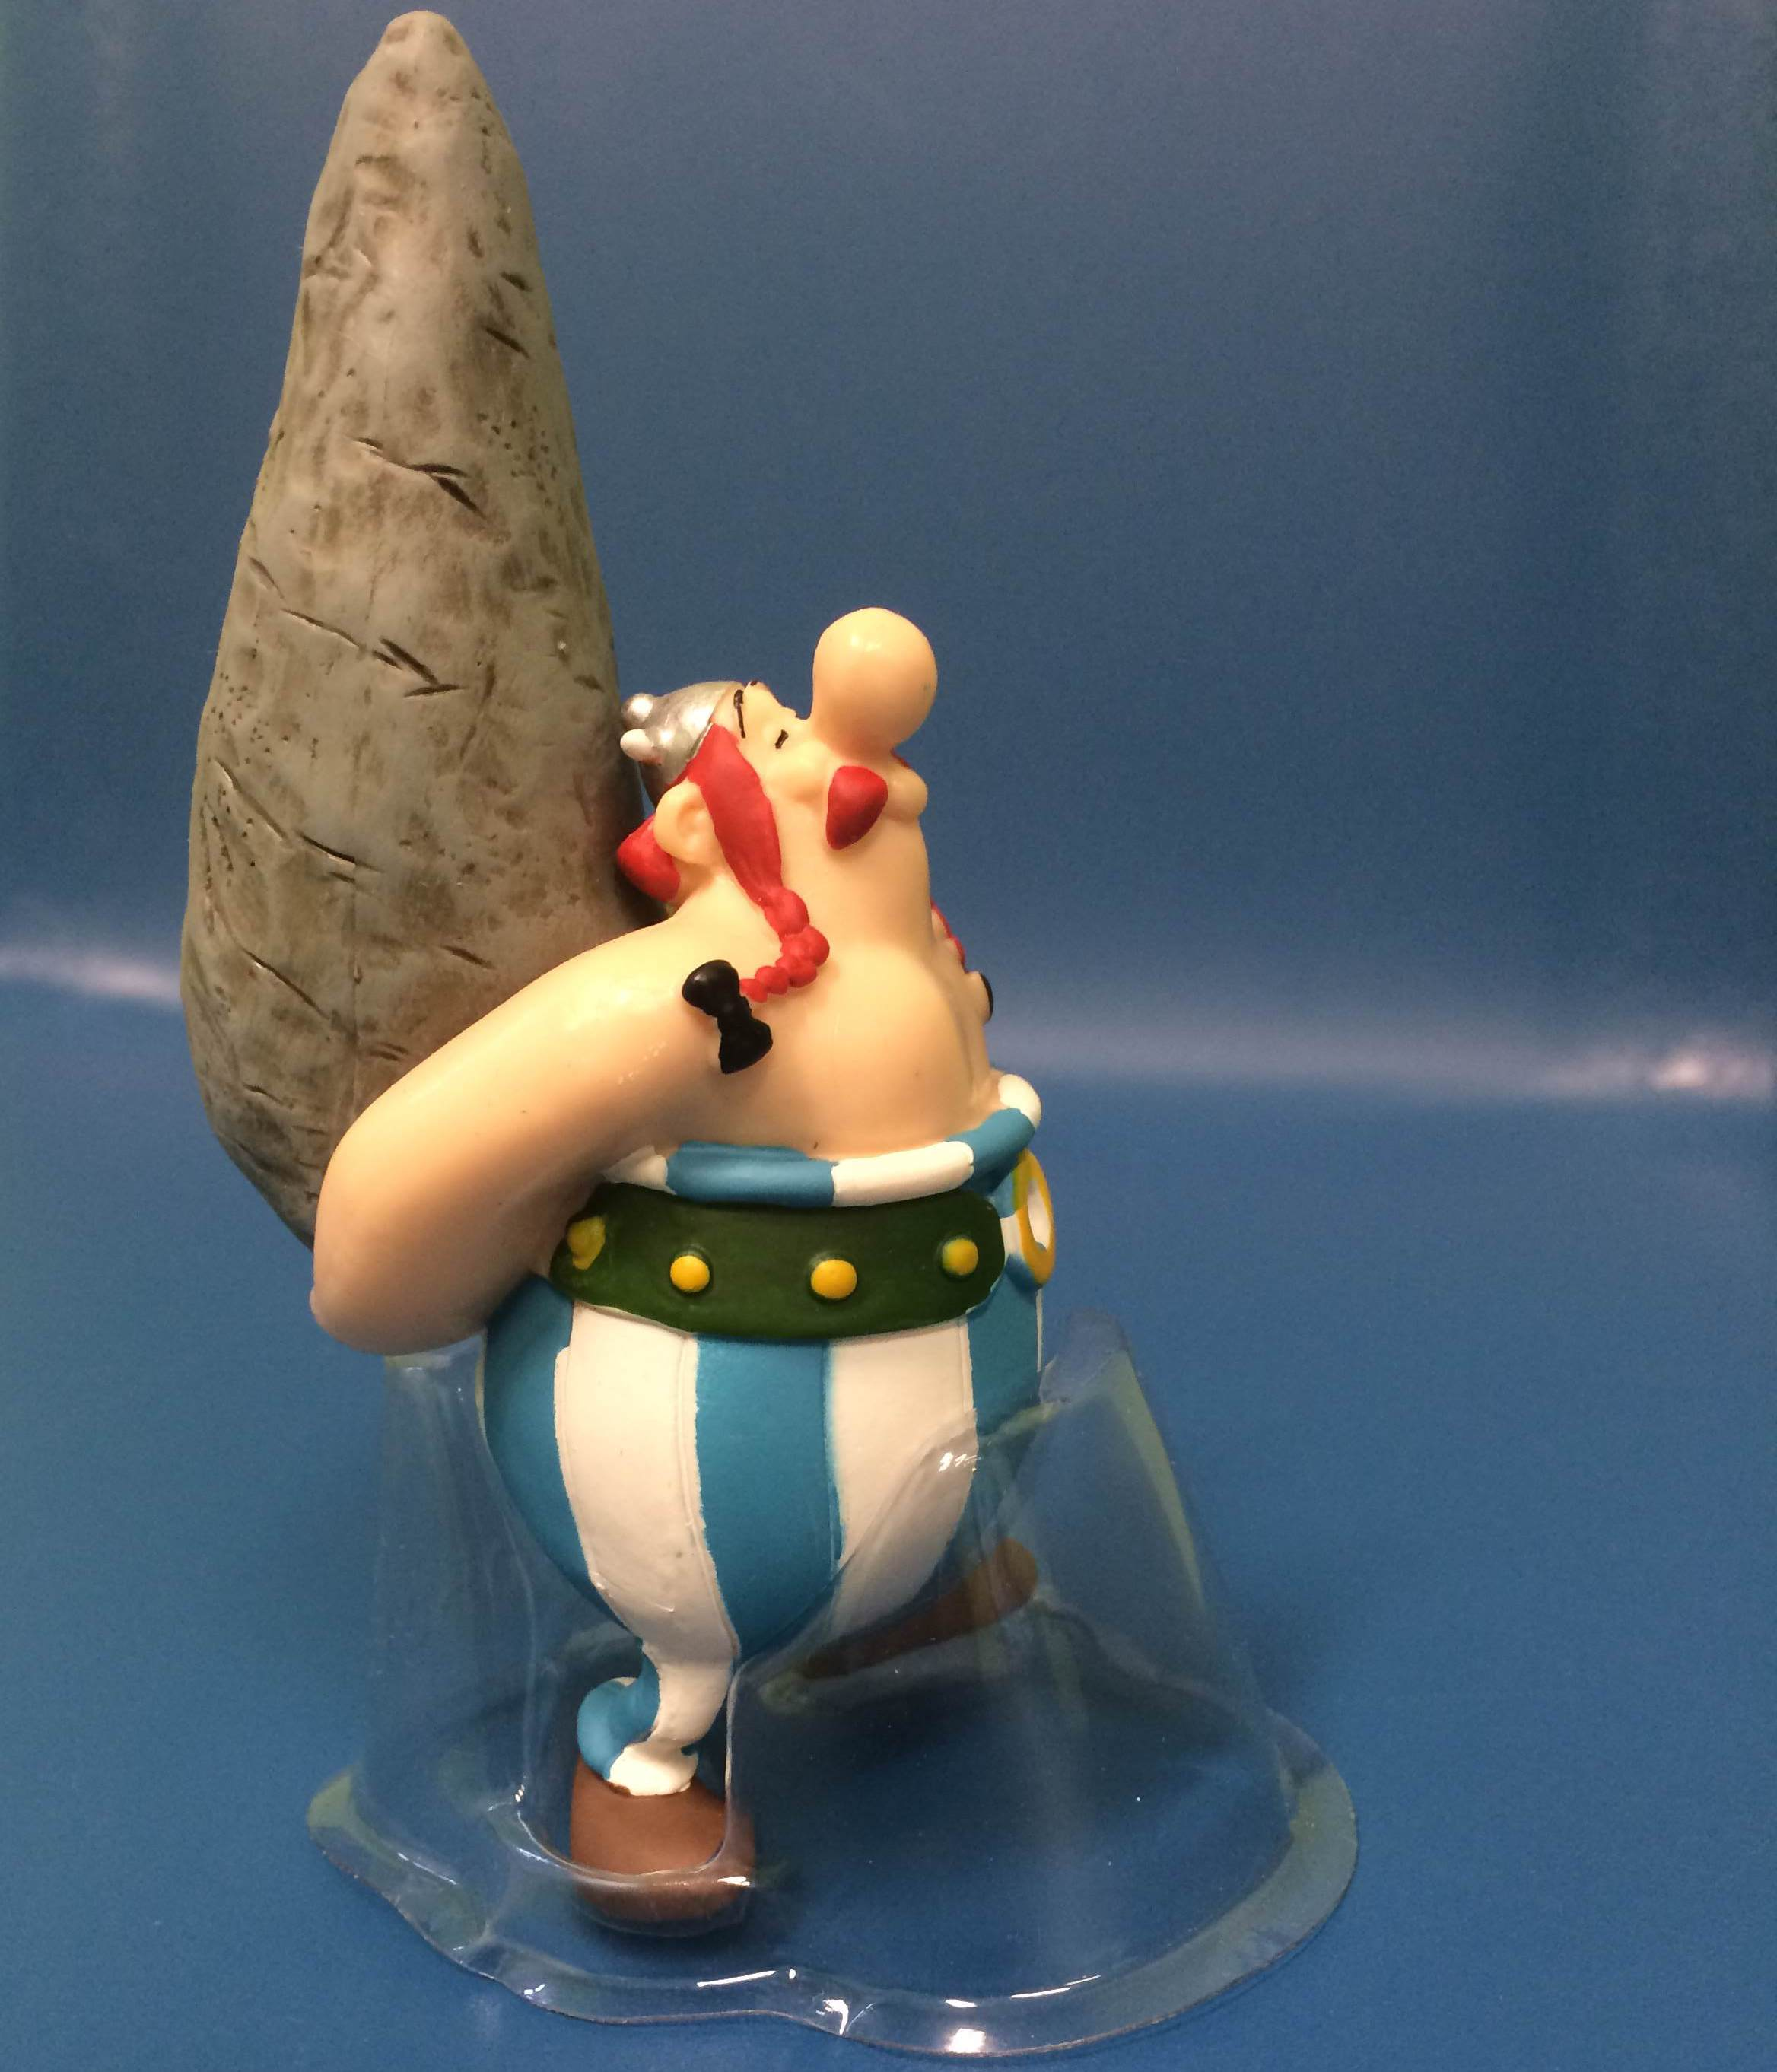
\includegraphics[scale=0.1334]{Obelix.jpg}
	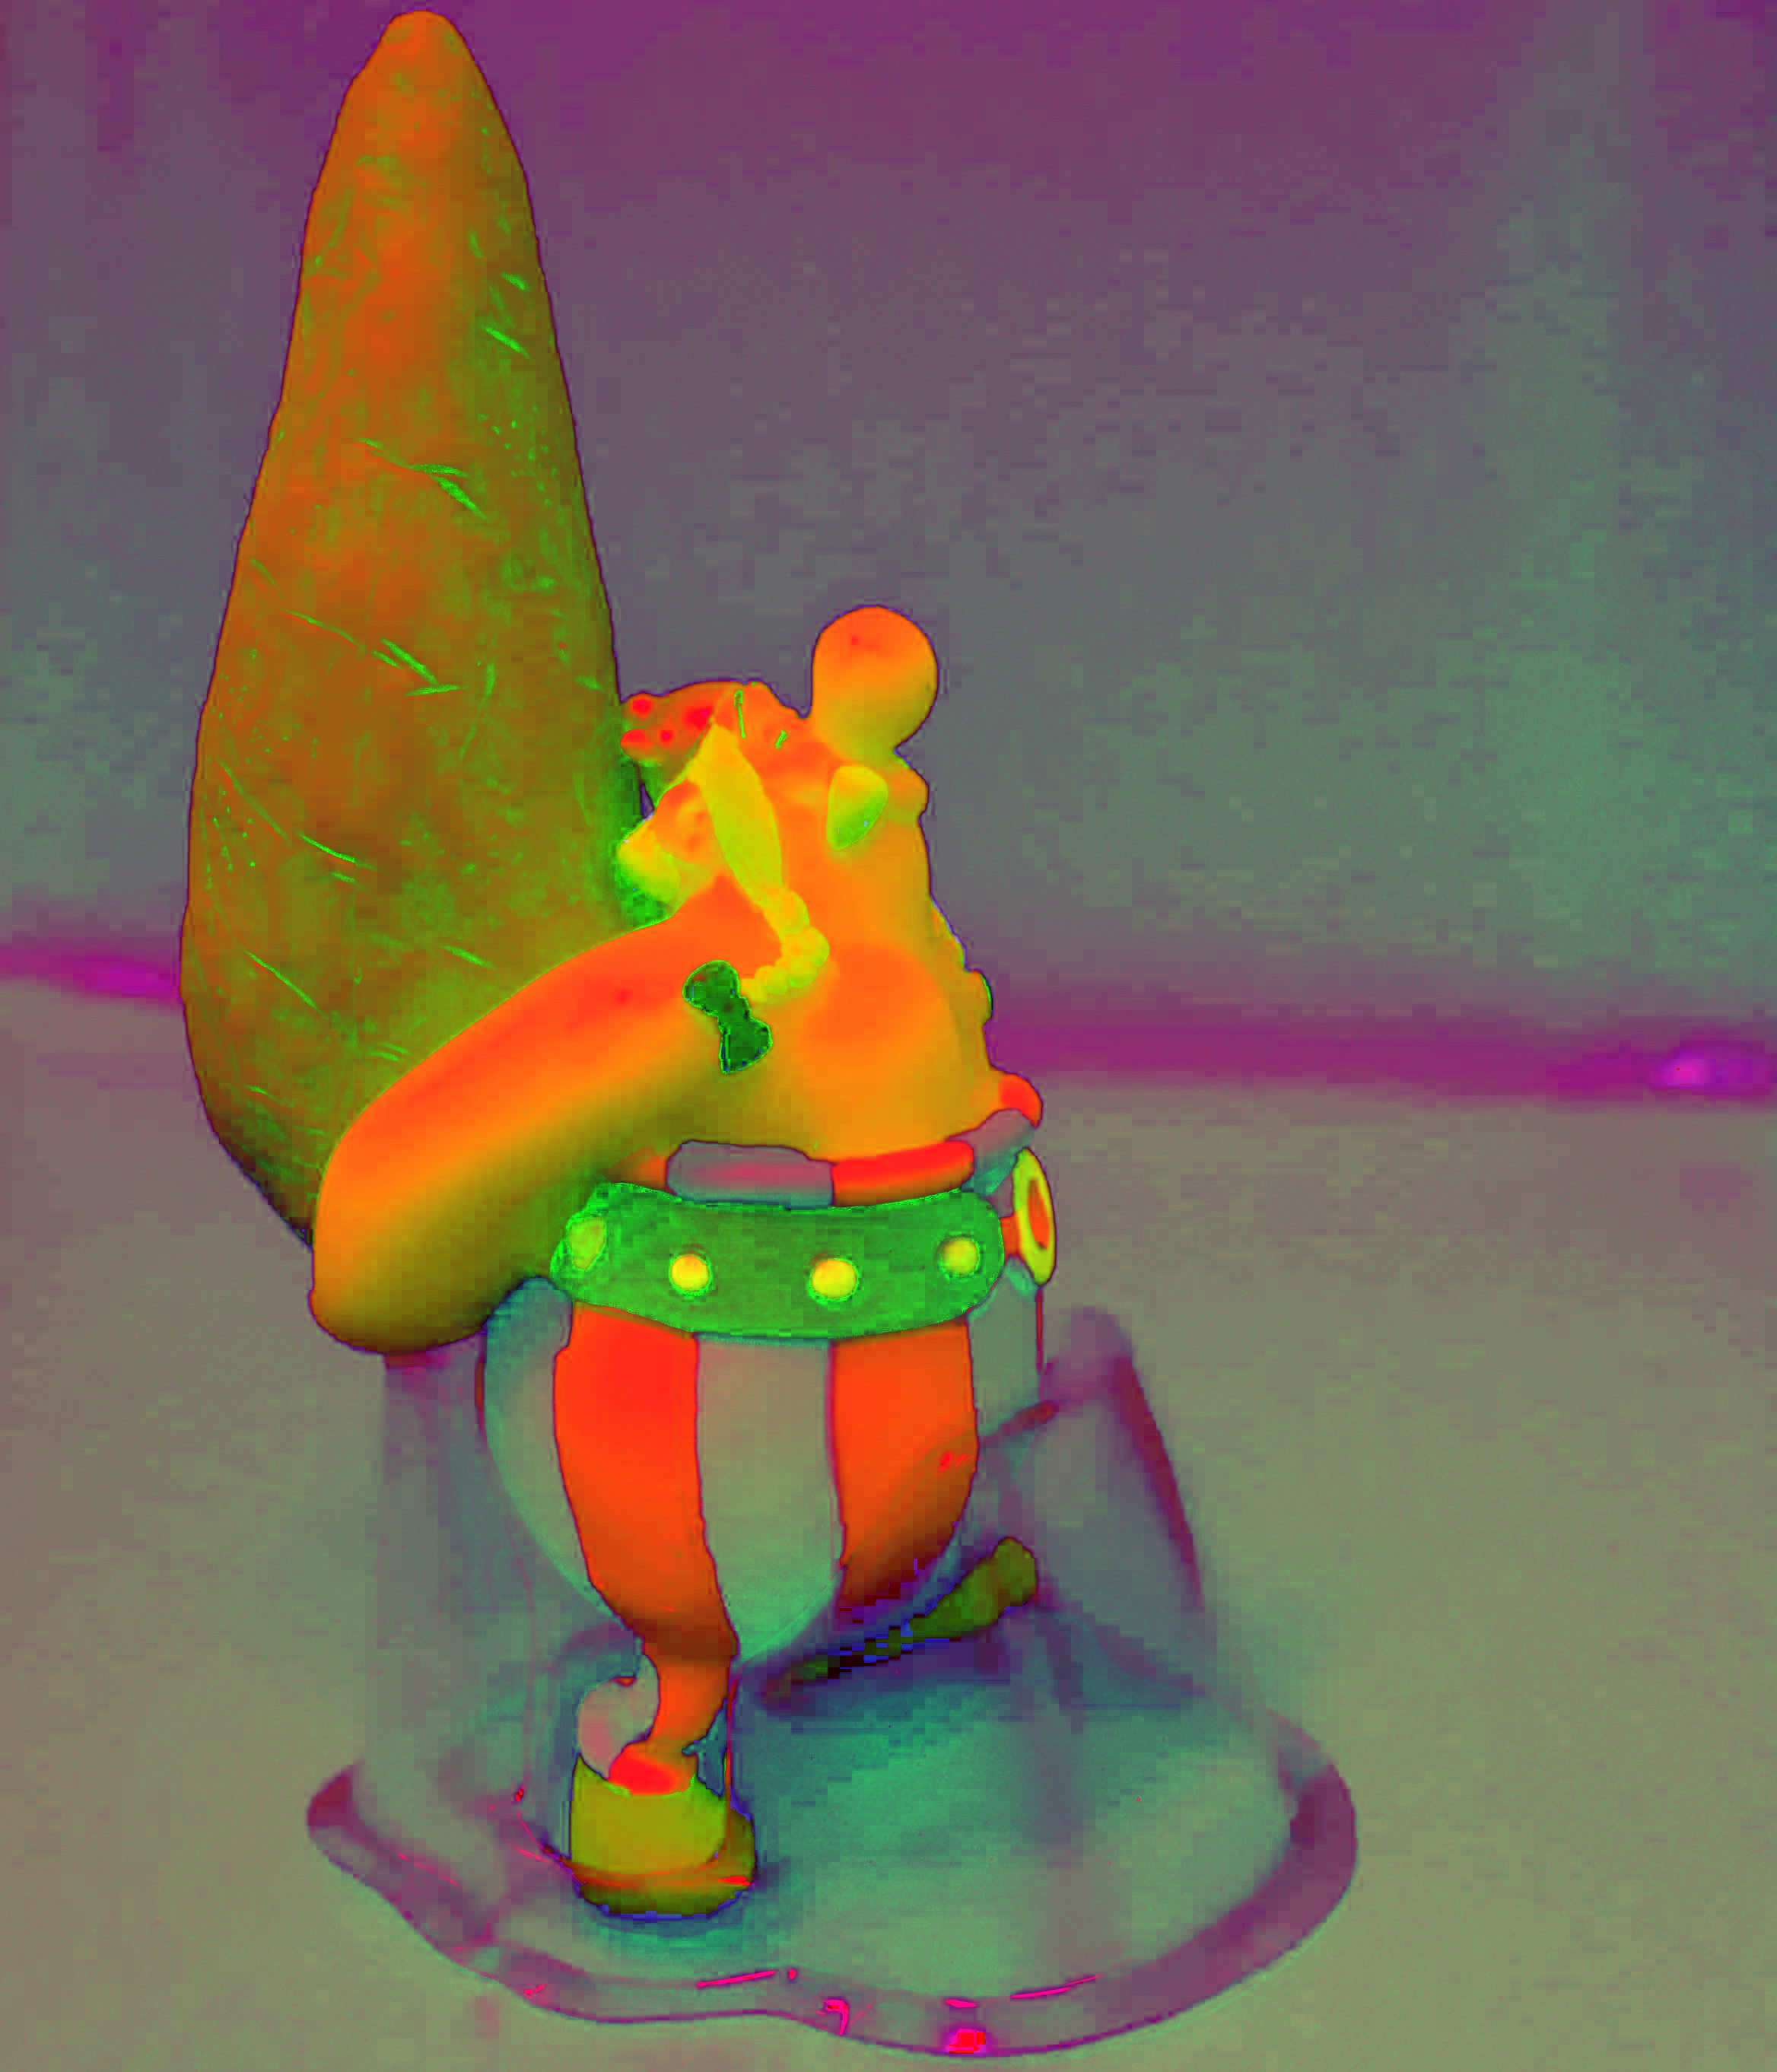
\includegraphics[scale=0.1]{obelx_hsv.jpg}
	\caption{The original image and HSV version of the image}
	\end{figure}
	\begin{figure}[H]
	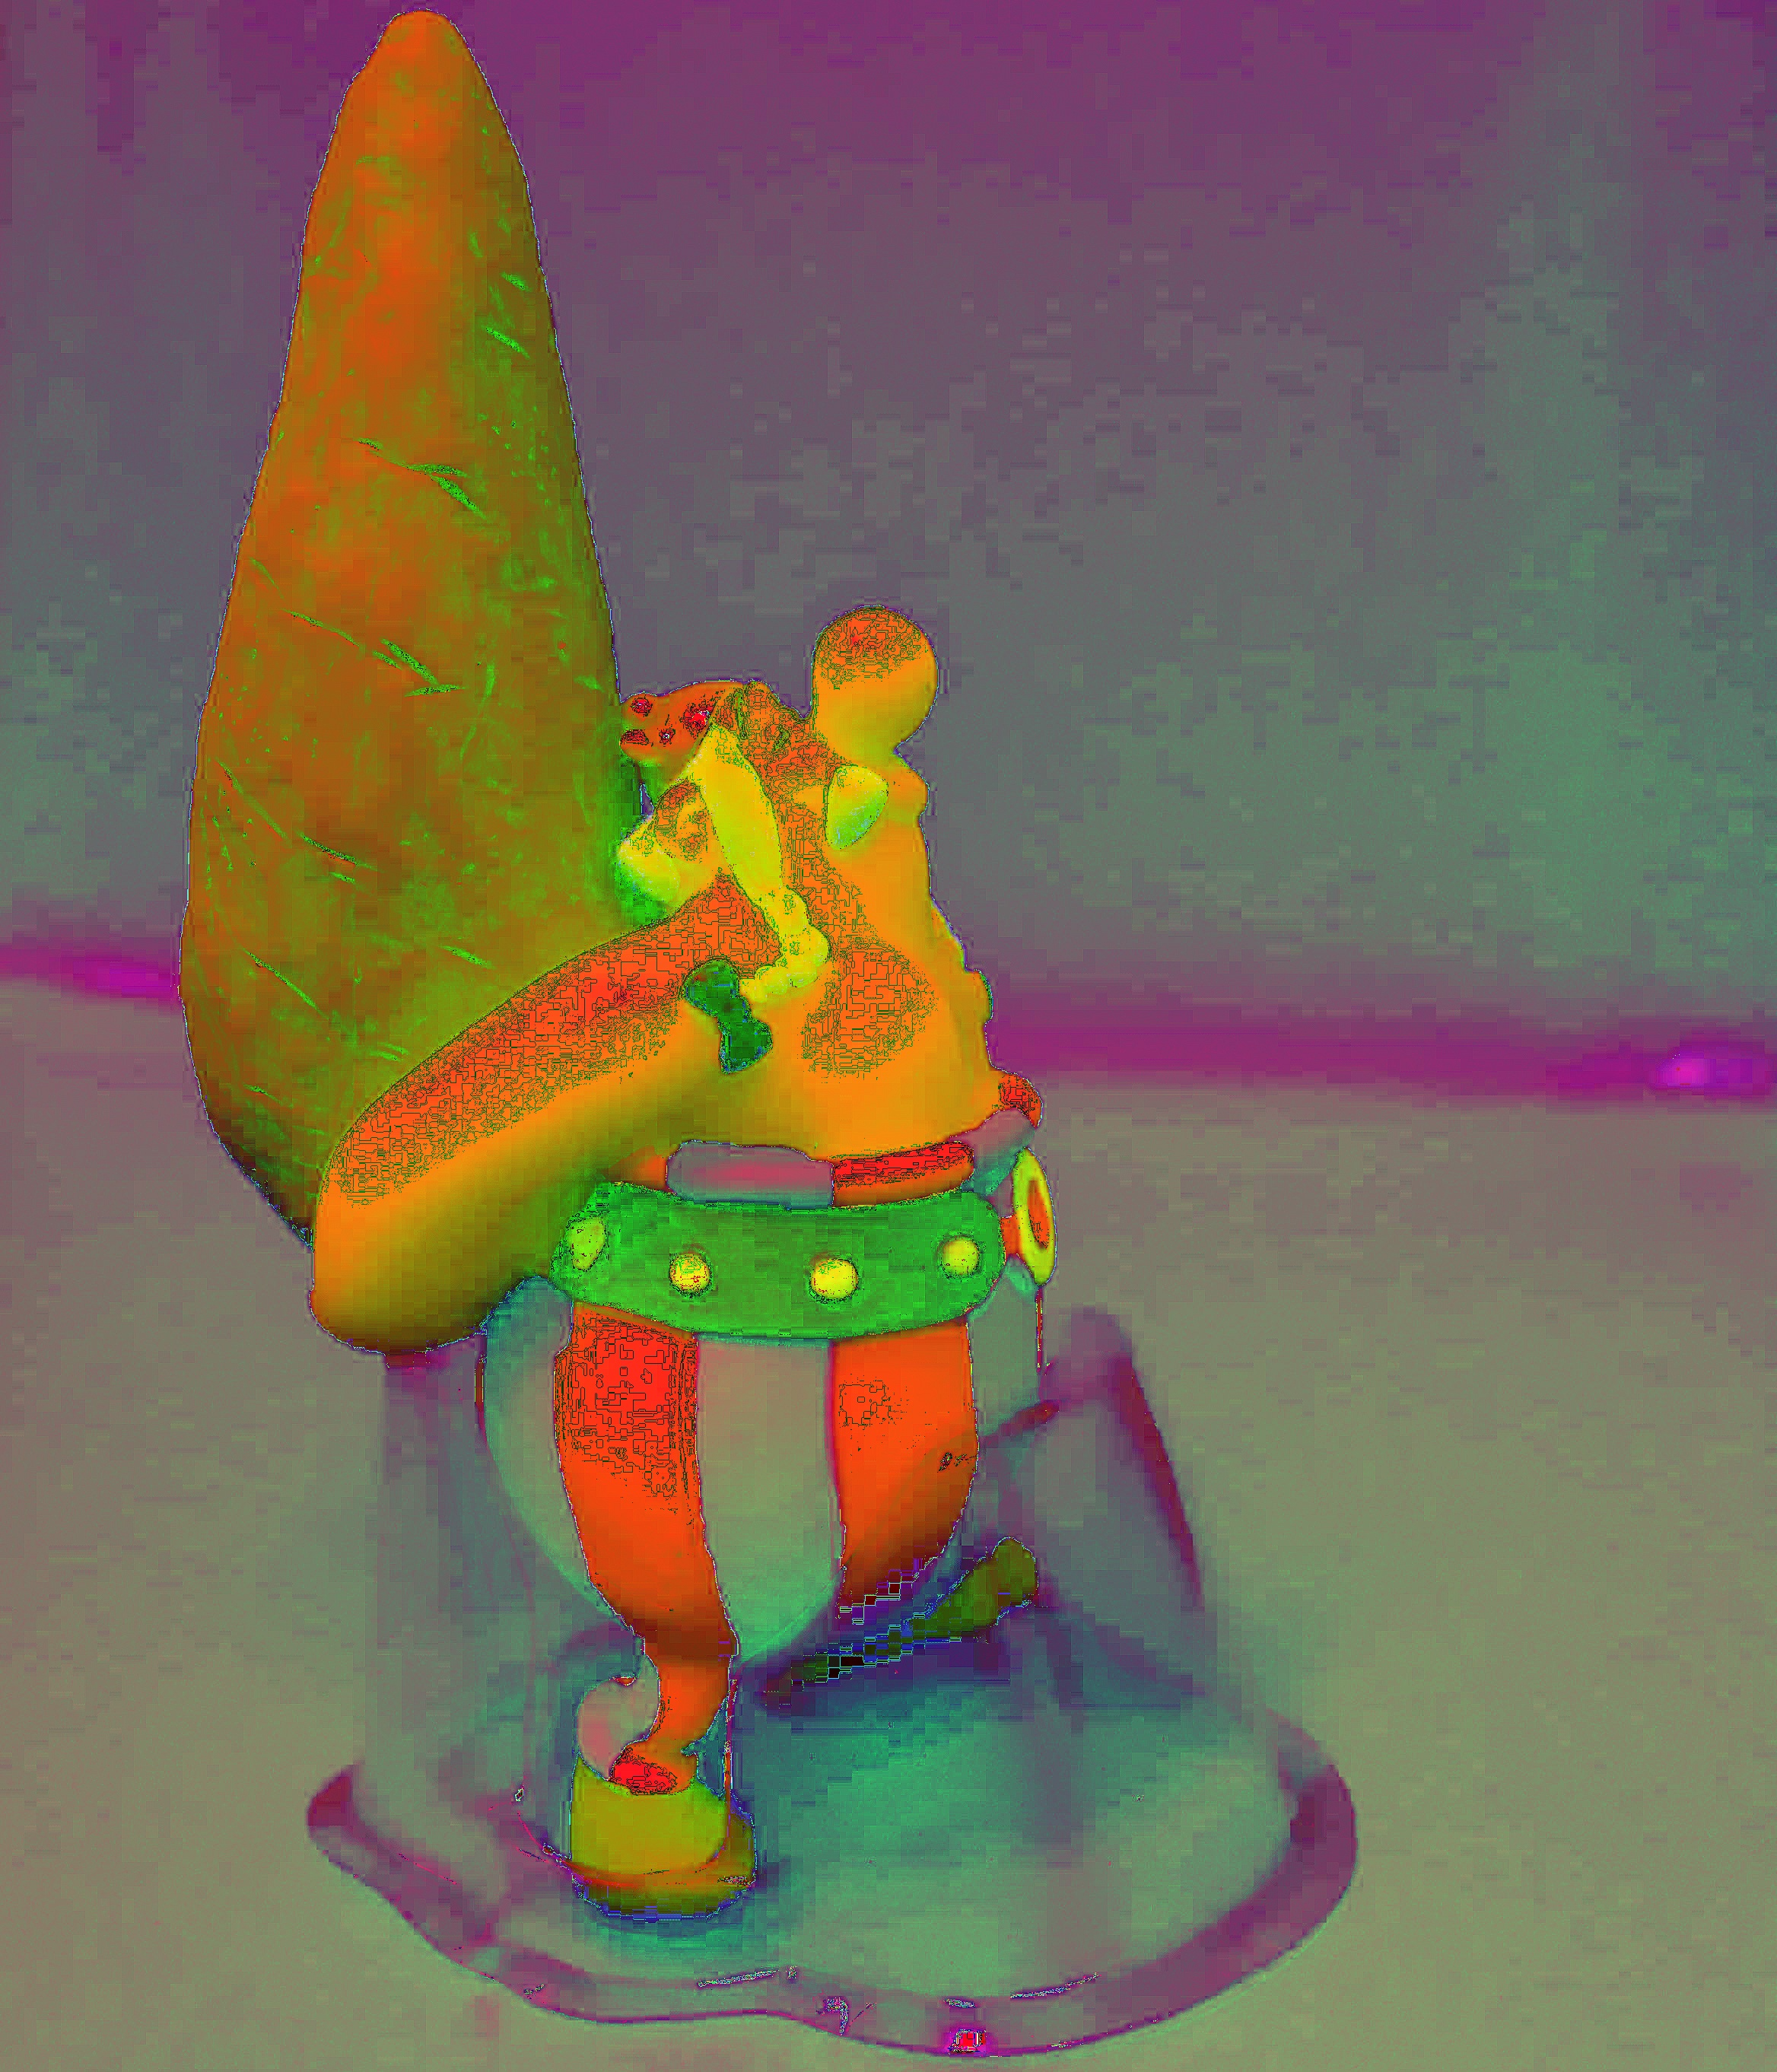
\includegraphics[scale=0.1]{obelx_hsv_sharpen_layerbylayer.jpg}
	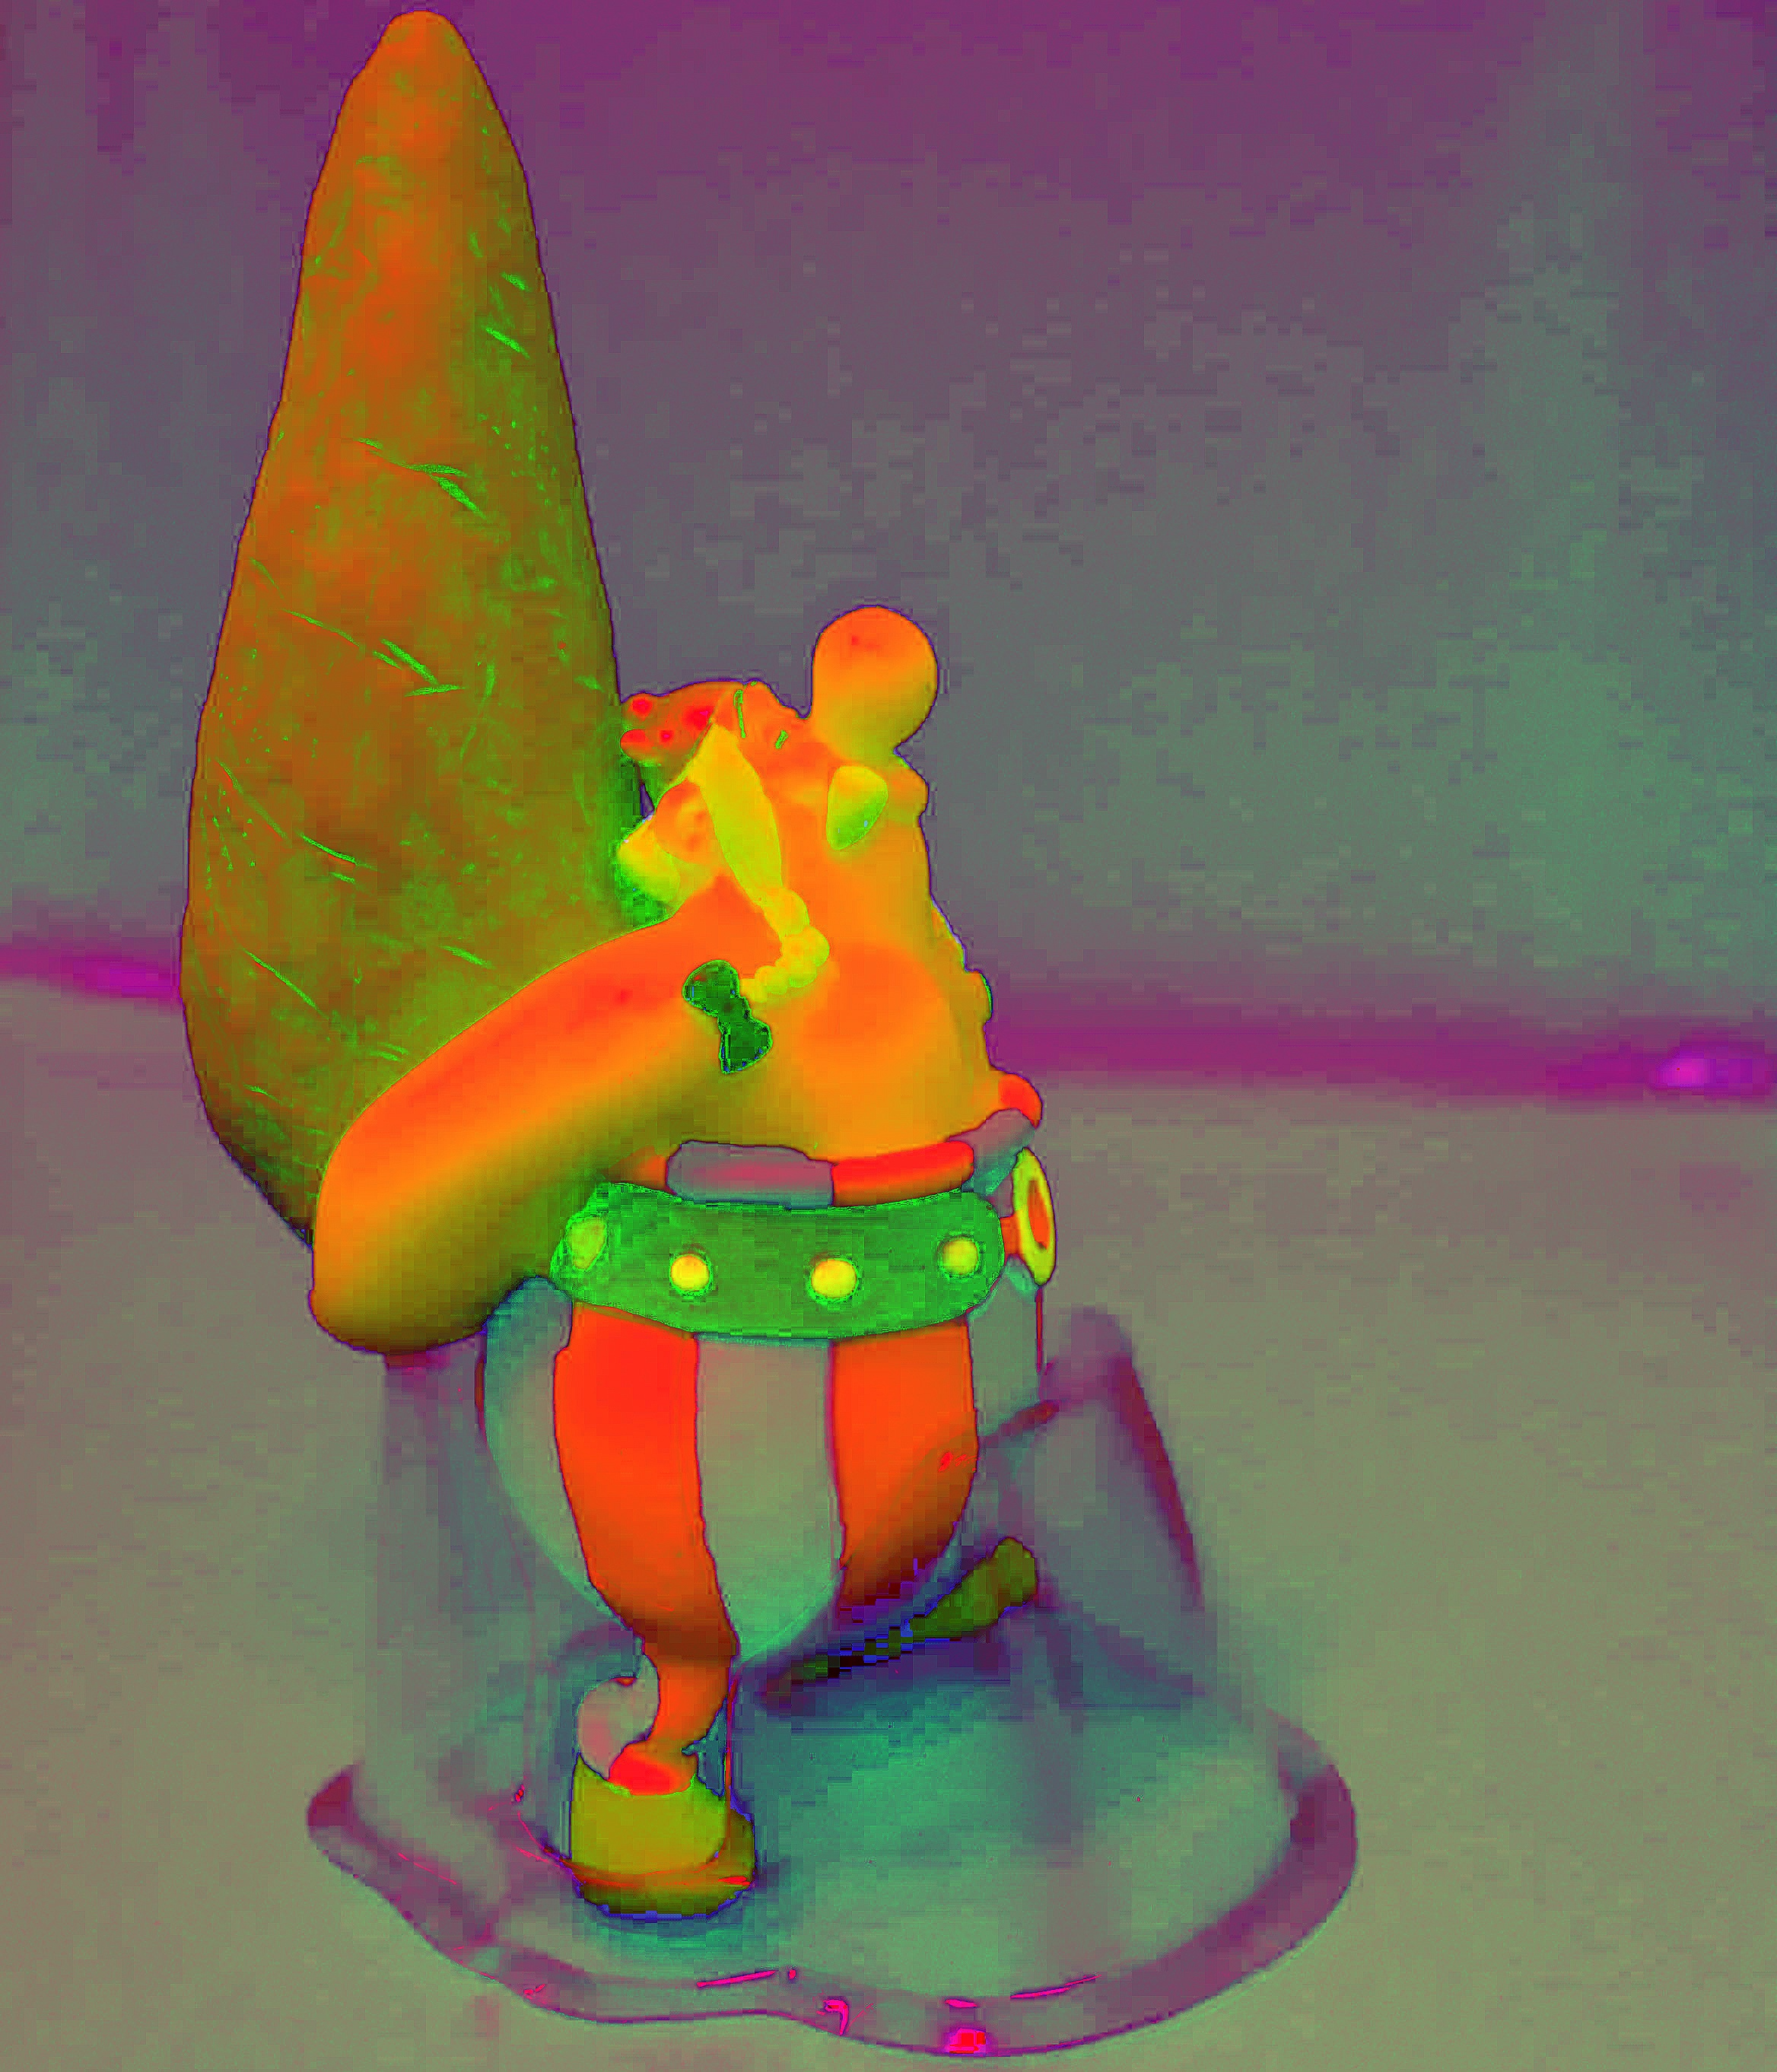
\includegraphics[scale=0.1]{obelx_hsv_sharpen_all.jpg}
	\caption{The left one is layer by layer , right all at once}
	\end{figure}
I used Laplacian sharpening to sharp the images. From the images we can notice that sharpening all of them at once is better I think one by one cause bias at some places where there is varied values in some layers which cause this noisy effect near the arm.
\section*{Code}
\subsection*{First Code}
At first I implemented the HSI method my self by this code :
\begin{lstlisting}[language=Python]
def RGTToHSIV3(img):
    print img.shape
    #Normailization
    img = np.array(img,dtype=np.float)
    thesum =np.sum(img,axis=2,dtype=np.float)
    img[:,:,0] = img[:,:,0]/thesum
    img[:,:,1] = img[:,:,1]/thesum
    img[:,:,2] = img[:,:,2]/thesum
    I = np.sum(img,axis=2)/3
    m = np.min(img,axis=2)
    #By default when divide by zero numpy assigen value of zero.
    S = 1-np.min(img,axis=2)/I
    numinator =img[:,:,2]-0.5*(img[:,:,0]+img[:,:,1]) #(R-1/2*(G+B))
    denum = np.sqrt(np.power(img[:,:,2]-img[:,:,1],2)+(img[:,:,2]-img[:,:,0])*(img[:,:,1]-img[:,:,0]))
    theta= np.degrees(np.arccos(numinator/(denum+0.00001)))
    coefg_geqb = img[:,:,1]>=img[:,:,0]
    coefg_g_b = img[:,:,0]>img[:,:,1]
    H = (coefg_geqb*theta+coefg_g_b*(360-theta))/360
    HSI = np.zeros(img.shape,dtype=float)
    HSI[:,:,0] = S
    HSI[:,:,1]=I
    HSI[:,:,2]=H
    return HSI
def HSItoRGB(img):
    R = np.ones((img.shape[0],img.shape[1]))
    G = np.ones((img.shape[0],img.shape[1]))
    B = np.zeros((img.shape[0],img.shape[1]))
    img[:,:,2]*=360
    for i in range (img.shape[0]):
        for j in range(img.shape[1]):
            S = img[i,j,0]
            I = img[i,j,1]
            H = img[i,j,2]
            if H==0:
                R[i,j]= I+2*I*S
                G[i,j]=I-I*S
                B[i,j] = I-I*S
            elif H>0 and H<120:
                R[i,j]= I + I*S*cos(H)/cos(60-H)
                G = I + I*S*[1 - cos(H)/cos(60-H)]
                B[i,j] = I-I*S
            elif H==120:
                R[i,j]= I-I*S
                G[i,j]=I+2*I*S
                B[i,j] = I-I*S
            elif H>120 and H<240:
                R[i,j] = I - I*S
                G[i,j] = I + I*S*cos(H-120)/cos(180-H)
                B[i,j] = I + I*S*[1 - cos(H-120)/cos(180-H)]
            elif H==240:
                R[i,j] = I - I*S
                G[i,j] = I - I*S
                B[i,j] = I + 2*I*S
            elif H>240 and H<360:
                R[i,j] = I + I*S*[1 - cos(H-240)/cos(300-H)]
                G[i,j] = I - I*S
                B[i,j] = I + I*S*cos(H-240)/cos(300-H)
    print R.shape
\end{lstlisting}
\section*{Second Code}
After that I used HSV (I sent an email about it and got a positive response)
\begin{lstlisting}[language=Python]
def readimg(name):
    return cv2.imread(name)

def laplacianSharpening(img):
    laplacian = cv2.Laplacian(img,cv2.CV_64F)
    #showimg(img-laplacian) 
    return (img-laplacian)
obelximg = readimg('Obelix.jpg')
obelximg_hsv = cv2.cvtColor(obelximg,cv2.COLOR_BGR2HSV)
cv2.imwrite('obelx_hsv.jpg',obelximg_hsv)
obeliximg_hsv_layerbylayer = obelximg_hsv.copy()
obeliximg_hsv_layerbylayer[:,:,0] = laplacianSharpening(obeliximg_hsv_layerbylayer[:,:,0])
obeliximg_hsv_layerbylayer[:,:,1] = laplacianSharpening(obeliximg_hsv_layerbylayer[:,:,1])
obeliximg_hsv_layerbylayer[:,:,2] = laplacianSharpening(obeliximg_hsv_layerbylayer[:,:,2])

cv2.imwrite('obelx_hsv_sharpen_layerbylayer.jpg',obeliximg_hsv_layerbylayer)
obelximg_hsv = laplacianSharpening(obelximg_hsv)
cv2.imwrite('obelx_hsv_sharpen_all.jpg',obelximg_hsv)
\end{lstlisting}
Used hints for sharpining from here\cite{1}\\
\textbf{Note:} All the Code,images,notes , tries , python etc.. files exist on \href{https://github.com/aqeel13932/IP/tree/master/hw5}{Github}
		\begin{thebibliography}{9}
			\bibitem{1}
		\href{https://github.com/abidrahmank/OpenCV2-Python-Tutorials/blob/master/source/py_tutorials/py_imgproc/py_gradients/py_gradients.rst}{Image Gradient}
		\end{thebibliography}
\end{document}